\documentclass[twoside]{book}

% Packages required by doxygen
\usepackage{fixltx2e}
\usepackage{calc}
\usepackage{doxygen}
\usepackage[export]{adjustbox} % also loads graphicx
\usepackage{graphicx}
\usepackage[utf8]{inputenc}
\usepackage{makeidx}
\usepackage{multicol}
\usepackage{multirow}
\PassOptionsToPackage{warn}{textcomp}
\usepackage{textcomp}
\usepackage[nointegrals]{wasysym}
\usepackage[table]{xcolor}

% NLS support packages
\usepackage[T2A]{fontenc}
\usepackage[magyar]{babel}

% Font selection
\usepackage[T1]{fontenc}
\usepackage[scaled=.90]{helvet}
\usepackage{courier}
\usepackage{amssymb}
\usepackage{sectsty}
\renewcommand{\familydefault}{\sfdefault}
\allsectionsfont{%
  \fontseries{bc}\selectfont%
  \color{darkgray}%
}
\renewcommand{\DoxyLabelFont}{%
  \fontseries{bc}\selectfont%
  \color{darkgray}%
}
\newcommand{\+}{\discretionary{\mbox{\scriptsize$\hookleftarrow$}}{}{}}

% Page & text layout
\usepackage{geometry}
\geometry{%
  a4paper,%
  top=2.5cm,%
  bottom=2.5cm,%
  left=2.5cm,%
  right=2.5cm%
}
\tolerance=750
\hfuzz=15pt
\hbadness=750
\setlength{\emergencystretch}{15pt}
\setlength{\parindent}{0cm}
\setlength{\parskip}{3ex plus 2ex minus 2ex}
\makeatletter
\renewcommand{\paragraph}{%
  \@startsection{paragraph}{4}{0ex}{-1.0ex}{1.0ex}{%
    \normalfont\normalsize\bfseries\SS@parafont%
  }%
}
\renewcommand{\subparagraph}{%
  \@startsection{subparagraph}{5}{0ex}{-1.0ex}{1.0ex}{%
    \normalfont\normalsize\bfseries\SS@subparafont%
  }%
}
\makeatother

% Headers & footers
\usepackage{fancyhdr}
\pagestyle{fancyplain}
\fancyhead[LE]{\fancyplain{}{\bfseries\thepage}}
\fancyhead[CE]{\fancyplain{}{}}
\fancyhead[RE]{\fancyplain{}{\bfseries\leftmark}}
\fancyhead[LO]{\fancyplain{}{\bfseries\rightmark}}
\fancyhead[CO]{\fancyplain{}{}}
\fancyhead[RO]{\fancyplain{}{\bfseries\thepage}}
\fancyfoot[LE]{\fancyplain{}{}}
\fancyfoot[CE]{\fancyplain{}{}}
\fancyfoot[RE]{\fancyplain{}{\bfseries\scriptsize Készítette Doxygen }}
\fancyfoot[LO]{\fancyplain{}{\bfseries\scriptsize Készítette Doxygen }}
\fancyfoot[CO]{\fancyplain{}{}}
\fancyfoot[RO]{\fancyplain{}{}}
\renewcommand{\footrulewidth}{0.4pt}
\renewcommand{\chaptermark}[1]{%
  \markboth{#1}{}%
}
\renewcommand{\sectionmark}[1]{%
  \markright{\thesection\ #1}%
}

% Indices & bibliography
\usepackage{natbib}
\usepackage[titles]{tocloft}
\setcounter{tocdepth}{3}
\setcounter{secnumdepth}{5}
\makeindex

% Hyperlinks (required, but should be loaded last)
\usepackage{ifpdf}
\ifpdf
  \usepackage[pdftex,pagebackref=true]{hyperref}
\else
  \usepackage[ps2pdf,pagebackref=true]{hyperref}
\fi
\hypersetup{%
  colorlinks=true,%
  linkcolor=blue,%
  citecolor=blue,%
  unicode%
}

% Custom commands
\newcommand{\clearemptydoublepage}{%
  \newpage{\pagestyle{empty}\cleardoublepage}%
}

\usepackage{caption}
\captionsetup{labelsep=space,justification=centering,font={bf},singlelinecheck=off,skip=4pt,position=top}

%===== C O N T E N T S =====

\begin{document}

% Titlepage & ToC
\hypersetup{pageanchor=false,
             bookmarksnumbered=true,
             pdfencoding=unicode
            }
\pagenumbering{alph}
\begin{titlepage}
\vspace*{7cm}
\begin{center}%
{\Large titkosito }\\
\vspace*{1cm}
{\large Készítette Doxygen 1.8.13}\\
\end{center}
\end{titlepage}
\clearemptydoublepage
\pagenumbering{roman}
\tableofcontents
\clearemptydoublepage
\pagenumbering{arabic}
\hypersetup{pageanchor=true}

%--- Begin generated contents ---
\chapter{Hierarchikus mutató}
\section{Osztályhierarchia}
Majdnem (de nem teljesen) betűrendbe szedett leszármazási lista\+:\begin{DoxyCompactList}
\item \contentsline{section}{call\+\_\+t}{\pageref{structcall__t}}{}
\item \contentsline{section}{Cipher}{\pageref{class_cipher}}{}
\begin{DoxyCompactList}
\item \contentsline{section}{Caesar\+Cipher}{\pageref{class_caesar_cipher}}{}
\item \contentsline{section}{X\+O\+R\+Cipher}{\pageref{class_x_o_r_cipher}}{}
\end{DoxyCompactList}
\item \contentsline{section}{Cipher\+String}{\pageref{class_cipher_string}}{}
\item \contentsline{section}{Test}{\pageref{class_test}}{}
\end{DoxyCompactList}

\chapter{Osztálymutató}
\section{Osztálylista}
Az összes osztály, struktúra, unió és interfész listája rövid leírásokkal\+:\begin{DoxyCompactList}
\item\contentsline{section}{\hyperlink{class_caesar_cipher}{Caesar\+Cipher} }{\pageref{class_caesar_cipher}}{}
\item\contentsline{section}{\hyperlink{structcall__t}{call\+\_\+t} }{\pageref{structcall__t}}{}
\item\contentsline{section}{\hyperlink{class_cipher}{Cipher} }{\pageref{class_cipher}}{}
\item\contentsline{section}{\hyperlink{class_cipher_string}{Cipher\+String} }{\pageref{class_cipher_string}}{}
\item\contentsline{section}{\hyperlink{class_test}{Test} }{\pageref{class_test}}{}
\item\contentsline{section}{\hyperlink{class_x_o_r_cipher}{X\+O\+R\+Cipher} }{\pageref{class_x_o_r_cipher}}{}
\end{DoxyCompactList}

\chapter{Osztályok dokumentációja}
\hypertarget{class_caesar_cipher}{}\section{Caesar\+Cipher osztályreferencia}
\label{class_caesar_cipher}\index{Caesar\+Cipher@{Caesar\+Cipher}}


{\ttfamily \#include $<$cipher.\+h$>$}

A Caesar\+Cipher osztály származási diagramja\+:\begin{figure}[H]
\begin{center}
\leavevmode
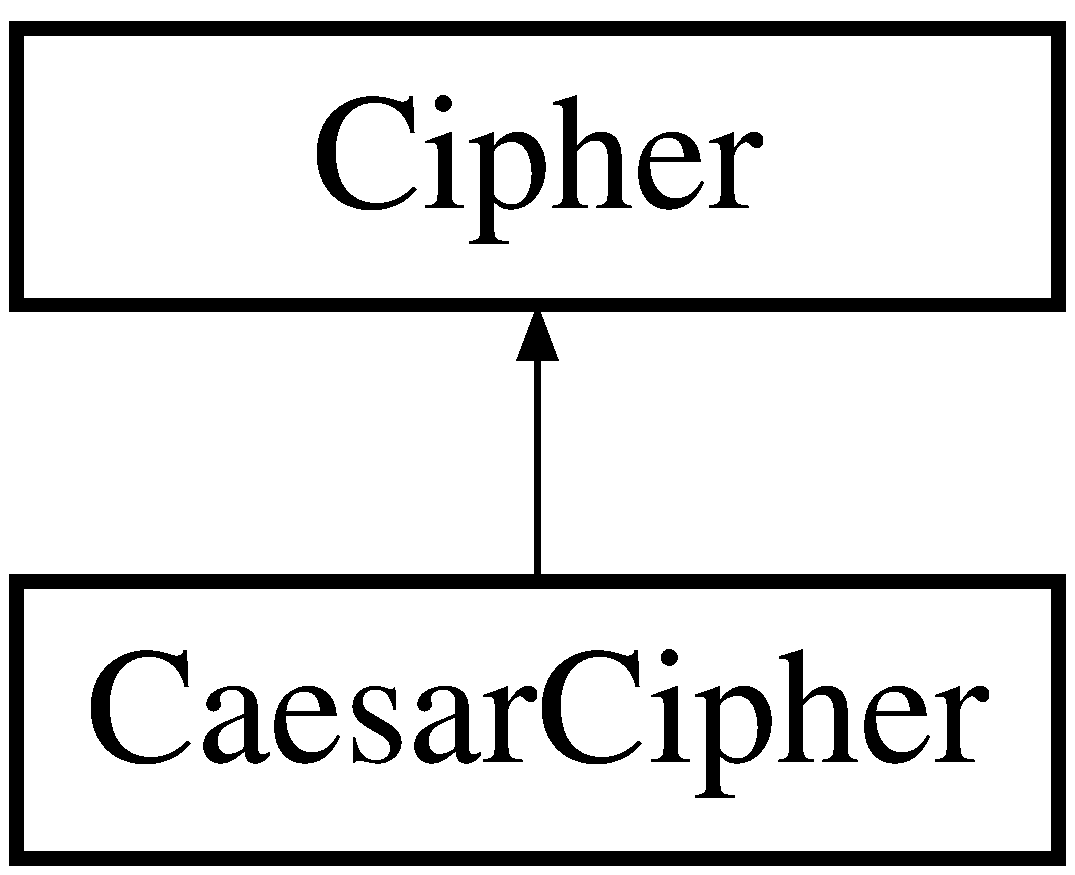
\includegraphics[height=2.000000cm]{class_caesar_cipher}
\end{center}
\end{figure}
\subsection*{Publikus tagfüggvények}
\begin{DoxyCompactItemize}
\item 
char $\ast$ \hyperlink{class_caesar_cipher_a394b73bf4835730e07f58945c0b0747a}{encrypt} (char $\ast$plain\+Text, char $\ast$cipher\+Key, int length)
\item 
char $\ast$ \hyperlink{class_caesar_cipher_a6362cea25d4027a1e1e9944739b4f33f}{decrypt} (char $\ast$cipher\+Text, char $\ast$cipher\+Key, int length)
\end{DoxyCompactItemize}


\subsection{Részletes leírás}
Caesar titkos�t� oszt�ly. � v�gzi a Caesar titkos�t�st �s visszafejt�st. 

\subsection{Tagfüggvények dokumentációja}
\mbox{\Hypertarget{class_caesar_cipher_a6362cea25d4027a1e1e9944739b4f33f}\label{class_caesar_cipher_a6362cea25d4027a1e1e9944739b4f33f}} 
\index{Caesar\+Cipher@{Caesar\+Cipher}!decrypt@{decrypt}}
\index{decrypt@{decrypt}!Caesar\+Cipher@{Caesar\+Cipher}}
\subsubsection{\texorpdfstring{decrypt()}{decrypt()}}
{\footnotesize\ttfamily char $\ast$ Caesar\+Cipher\+::decrypt (\begin{DoxyParamCaption}\item[{char $\ast$}]{cipher\+Text,  }\item[{char $\ast$}]{cipher\+Key,  }\item[{int}]{length }\end{DoxyParamCaption})\hspace{0.3cm}{\ttfamily [virtual]}}

Az abstract oszt�ly virtu�lis visszafejt� met�dusa. A param�ter�l kapott �rt�ket a param�ter�l kapott titkos kulccsal visszafejti eredeti �llapot�ba.


\begin{DoxyParams}{Paraméterek}
{\em cipher\+Text} & A titkos�tott sz�veg \\
\hline
{\em cipher\+Key} & A titkos kulcs \\
\hline
{\em length} & A titkos�tott sz�veg hossza \\
\hline
\end{DoxyParams}
\begin{DoxyReturn}{Visszatérési érték}
A visszafejtett sz�veg 
\end{DoxyReturn}


Megvalósítja a következőket\+: \hyperlink{class_cipher_a39b1608e01f73f75ee248ef566aa44f9}{Cipher}.

\mbox{\Hypertarget{class_caesar_cipher_a394b73bf4835730e07f58945c0b0747a}\label{class_caesar_cipher_a394b73bf4835730e07f58945c0b0747a}} 
\index{Caesar\+Cipher@{Caesar\+Cipher}!encrypt@{encrypt}}
\index{encrypt@{encrypt}!Caesar\+Cipher@{Caesar\+Cipher}}
\subsubsection{\texorpdfstring{encrypt()}{encrypt()}}
{\footnotesize\ttfamily char $\ast$ Caesar\+Cipher\+::encrypt (\begin{DoxyParamCaption}\item[{char $\ast$}]{plain\+Text,  }\item[{char $\ast$}]{cipher\+Key,  }\item[{int}]{length }\end{DoxyParamCaption})\hspace{0.3cm}{\ttfamily [virtual]}}

Az abstract oszt�ly virtu�lis titkos�t� met�dusa. A param�ter�l kapott �rt�ket a szint�n param�ter�l kapott titkos kulccsal titkos�tja.


\begin{DoxyParams}{Paraméterek}
{\em plain\+Text} & A titkos�tand� sz�veg \\
\hline
{\em cipher\+Key} & A titkos kulcs \\
\hline
{\em length} & A titkos�tand� sz�veg hossza \\
\hline
\end{DoxyParams}
\begin{DoxyReturn}{Visszatérési érték}
A titkos�tott sz�veg 
\end{DoxyReturn}


Megvalósítja a következőket\+: \hyperlink{class_cipher_a8a1970fdcb363529590299f14a6f2571}{Cipher}.



Ez a dokumentáció az osztályról a következő fájlok alapján készült\+:\begin{DoxyCompactItemize}
\item 
cipher.\+h\item 
cipher.\+cpp\end{DoxyCompactItemize}

\hypertarget{structcall__t}{}\section{call\+\_\+t struktúrareferencia}
\label{structcall__t}\index{call\+\_\+t@{call\+\_\+t}}
\subsection*{Publikus attribútumok}
\begin{DoxyCompactItemize}
\item 
\mbox{\Hypertarget{structcall__t_a59d4e803f2e254dc5ceeb9c1bfcc9355}\label{structcall__t_a59d4e803f2e254dc5ceeb9c1bfcc9355}} 
int {\bfseries f}
\item 
\mbox{\Hypertarget{structcall__t_aaa4f0e556289bbf4da414897b10e0916}\label{structcall__t_aaa4f0e556289bbf4da414897b10e0916}} 
int {\bfseries line}
\item 
\mbox{\Hypertarget{structcall__t_a24e185188a17e272396e118640672aba}\label{structcall__t_a24e185188a17e272396e118640672aba}} 
char $\ast$ {\bfseries par\+\_\+txt}
\item 
\mbox{\Hypertarget{structcall__t_a97629ec51d024396221fe7d48c84859a}\label{structcall__t_a97629ec51d024396221fe7d48c84859a}} 
char $\ast$ {\bfseries file}
\end{DoxyCompactItemize}


Ez a dokumentáció a struktúráról a következő fájl alapján készült\+:\begin{DoxyCompactItemize}
\item 
memtrace.\+cpp\end{DoxyCompactItemize}

\hypertarget{class_cipher}{}\section{Cipher osztályreferencia}
\label{class_cipher}\index{Cipher@{Cipher}}


{\ttfamily \#include $<$cipher.\+h$>$}

A Cipher osztály származási diagramja\+:\begin{figure}[H]
\begin{center}
\leavevmode
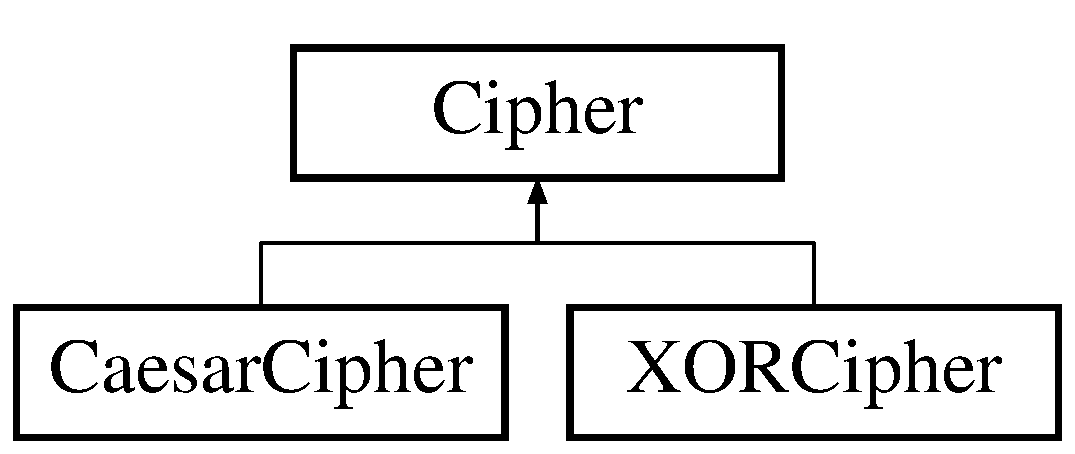
\includegraphics[height=2.000000cm]{class_cipher}
\end{center}
\end{figure}
\subsection*{Publikus tagfüggvények}
\begin{DoxyCompactItemize}
\item 
virtual char $\ast$ \hyperlink{class_cipher_a8a1970fdcb363529590299f14a6f2571}{encrypt} (char $\ast$plain\+Text, char $\ast$cipher\+Key, int length)=0
\item 
virtual char $\ast$ \hyperlink{class_cipher_a39b1608e01f73f75ee248ef566aa44f9}{decrypt} (char $\ast$cipher\+Text, char $\ast$cipher\+Key, int length)=0
\end{DoxyCompactItemize}


\subsection{Részletes leírás}
Abstract oszt�ly a heterog�n kollekci� kezel�s�hez. Minden titkos�t� oszt�ly �se. 

\subsection{Tagfüggvények dokumentációja}
\mbox{\Hypertarget{class_cipher_a39b1608e01f73f75ee248ef566aa44f9}\label{class_cipher_a39b1608e01f73f75ee248ef566aa44f9}} 
\index{Cipher@{Cipher}!decrypt@{decrypt}}
\index{decrypt@{decrypt}!Cipher@{Cipher}}
\subsubsection{\texorpdfstring{decrypt()}{decrypt()}}
{\footnotesize\ttfamily virtual char$\ast$ Cipher\+::decrypt (\begin{DoxyParamCaption}\item[{char $\ast$}]{cipher\+Text,  }\item[{char $\ast$}]{cipher\+Key,  }\item[{int}]{length }\end{DoxyParamCaption})\hspace{0.3cm}{\ttfamily [pure virtual]}}

Az abstract oszt�ly virtu�lis visszafejt� met�dusa. A param�ter�l kapott �rt�ket a param�ter�l kapott titkos kulccsal visszafejti eredeti �llapot�ba.


\begin{DoxyParams}{Paraméterek}
{\em cipher\+Text} & A titkos�tott sz�veg \\
\hline
{\em cipher\+Key} & A titkos kulcs \\
\hline
{\em length} & A titkos�tott sz�veg hossza \\
\hline
\end{DoxyParams}
\begin{DoxyReturn}{Visszatérési érték}
A visszafejtett sz�veg 
\end{DoxyReturn}


Megvalósítják a következők\+: \hyperlink{class_x_o_r_cipher_ab3afeef39c53f0345163a6e46aac25b3}{X\+O\+R\+Cipher} és \hyperlink{class_caesar_cipher_a6362cea25d4027a1e1e9944739b4f33f}{Caesar\+Cipher}.

\mbox{\Hypertarget{class_cipher_a8a1970fdcb363529590299f14a6f2571}\label{class_cipher_a8a1970fdcb363529590299f14a6f2571}} 
\index{Cipher@{Cipher}!encrypt@{encrypt}}
\index{encrypt@{encrypt}!Cipher@{Cipher}}
\subsubsection{\texorpdfstring{encrypt()}{encrypt()}}
{\footnotesize\ttfamily virtual char$\ast$ Cipher\+::encrypt (\begin{DoxyParamCaption}\item[{char $\ast$}]{plain\+Text,  }\item[{char $\ast$}]{cipher\+Key,  }\item[{int}]{length }\end{DoxyParamCaption})\hspace{0.3cm}{\ttfamily [pure virtual]}}

Az abstract oszt�ly virtu�lis titkos�t� met�dusa. A param�ter�l kapott �rt�ket a szint�n param�ter�l kapott titkos kulccsal titkos�tja.


\begin{DoxyParams}{Paraméterek}
{\em plain\+Text} & A titkos�tand� sz�veg \\
\hline
{\em cipher\+Key} & A titkos kulcs \\
\hline
{\em length} & A titkos�tand� sz�veg hossza \\
\hline
\end{DoxyParams}
\begin{DoxyReturn}{Visszatérési érték}
A titkos�tott sz�veg 
\end{DoxyReturn}


Megvalósítják a következők\+: \hyperlink{class_x_o_r_cipher_ac8ac09a4fcac428386935c31dea03768}{X\+O\+R\+Cipher} és \hyperlink{class_caesar_cipher_a394b73bf4835730e07f58945c0b0747a}{Caesar\+Cipher}.



Ez a dokumentáció az osztályról a következő fájl alapján készült\+:\begin{DoxyCompactItemize}
\item 
cipher.\+h\end{DoxyCompactItemize}

\hypertarget{class_cipher_string}{}\section{Cipher\+String osztályreferencia}
\label{class_cipher_string}\index{Cipher\+String@{Cipher\+String}}


{\ttfamily \#include $<$cipherstring.\+h$>$}

\subsection*{Publikus tagfüggvények}
\begin{DoxyCompactItemize}
\item 
\hyperlink{class_cipher_string_a78d5c6bcc232f0c2cde34d5706107127}{Cipher\+String} ()
\item 
char $\ast$ \hyperlink{class_cipher_string_ad697651cb43128c9f980a00f2fd31c69}{caesar\+Encrypt} (char $\ast$plain\+String\+In, char $\ast$cipher\+Key)
\item 
char $\ast$ \hyperlink{class_cipher_string_abb9c46f5902c8d3cf58f1adbbe571e58}{xor\+Encrypt} (char $\ast$plain\+String\+In, char $\ast$cipher\+Key)
\item 
char $\ast$ \hyperlink{class_cipher_string_a06310ff798cab137ae7faa769fc512d8}{caesar\+Decrypt} (char $\ast$cipher\+Key)
\item 
char $\ast$ \hyperlink{class_cipher_string_a9d8689809d1e4e77867466e56335977d}{xor\+Decrypt} (char $\ast$cipher\+Key)
\item 
virtual \hyperlink{class_cipher_string_a805b365286a97e096db9c04b555f3ef9}{$\sim$\+Cipher\+String} ()
\end{DoxyCompactItemize}


\subsection{Részletes leírás}
\hyperlink{class_cipher}{Cipher} String oszt�ály. Ő tárolja a titkosított szöveget és a hosszát. Referenciával rendelkezik a titkosítákra. Az ő segítségükkel titkosítja a kapott szöveget. 

\subsection{Konstruktorok és destruktorok dokumentációja}
\mbox{\Hypertarget{class_cipher_string_a78d5c6bcc232f0c2cde34d5706107127}\label{class_cipher_string_a78d5c6bcc232f0c2cde34d5706107127}} 
\index{Cipher\+String@{Cipher\+String}!Cipher\+String@{Cipher\+String}}
\index{Cipher\+String@{Cipher\+String}!Cipher\+String@{Cipher\+String}}
\subsubsection{\texorpdfstring{Cipher\+String()}{CipherString()}}
{\footnotesize\ttfamily Cipher\+String\+::\+Cipher\+String (\begin{DoxyParamCaption}{ }\end{DoxyParamCaption})\hspace{0.3cm}{\ttfamily [inline]}}

Publikus, paraméter nélküli konstruktor \mbox{\Hypertarget{class_cipher_string_a805b365286a97e096db9c04b555f3ef9}\label{class_cipher_string_a805b365286a97e096db9c04b555f3ef9}} 
\index{Cipher\+String@{Cipher\+String}!````~Cipher\+String@{$\sim$\+Cipher\+String}}
\index{````~Cipher\+String@{$\sim$\+Cipher\+String}!Cipher\+String@{Cipher\+String}}
\subsubsection{\texorpdfstring{$\sim$\+Cipher\+String()}{~CipherString()}}
{\footnotesize\ttfamily virtual Cipher\+String\+::$\sim$\+Cipher\+String (\begin{DoxyParamCaption}{ }\end{DoxyParamCaption})\hspace{0.3cm}{\ttfamily [inline]}, {\ttfamily [virtual]}}

Destruktor. 

\subsection{Tagfüggvények dokumentációja}
\mbox{\Hypertarget{class_cipher_string_a06310ff798cab137ae7faa769fc512d8}\label{class_cipher_string_a06310ff798cab137ae7faa769fc512d8}} 
\index{Cipher\+String@{Cipher\+String}!caesar\+Decrypt@{caesar\+Decrypt}}
\index{caesar\+Decrypt@{caesar\+Decrypt}!Cipher\+String@{Cipher\+String}}
\subsubsection{\texorpdfstring{caesar\+Decrypt()}{caesarDecrypt()}}
{\footnotesize\ttfamily char $\ast$ Cipher\+String\+::caesar\+Decrypt (\begin{DoxyParamCaption}\item[{char $\ast$}]{cipher\+Key }\end{DoxyParamCaption})}

Caesar visszafejtő metódus, a paraméterül kapott kulccsal visszafejti az osztályban tárolt titkos szöveget.


\begin{DoxyParams}{Paraméterek}
{\em cipher\+Key} & A titkos kulcs \\
\hline
\end{DoxyParams}
\begin{DoxyReturn}{Visszatérési érték}
Az osztály által tárolt szöveg visszafejtett változata 
\end{DoxyReturn}
\mbox{\Hypertarget{class_cipher_string_ad697651cb43128c9f980a00f2fd31c69}\label{class_cipher_string_ad697651cb43128c9f980a00f2fd31c69}} 
\index{Cipher\+String@{Cipher\+String}!caesar\+Encrypt@{caesar\+Encrypt}}
\index{caesar\+Encrypt@{caesar\+Encrypt}!Cipher\+String@{Cipher\+String}}
\subsubsection{\texorpdfstring{caesar\+Encrypt()}{caesarEncrypt()}}
{\footnotesize\ttfamily char $\ast$ Cipher\+String\+::caesar\+Encrypt (\begin{DoxyParamCaption}\item[{char $\ast$}]{plain\+String\+In,  }\item[{char $\ast$}]{cipher\+Key }\end{DoxyParamCaption})}

Caesar Titkosító metódus, a paraméterül kapott értéket a szintén paraméterül kapott kulccsal titkosítja.


\begin{DoxyParams}{Paraméterek}
{\em plain\+String\+In} & A titkosítandó szüöveg \\
\hline
{\em cipher\+Key} & A titkos kulcs \\
\hline
\end{DoxyParams}
\begin{DoxyReturn}{Visszatérési érték}
A titkosított szöveg 
\end{DoxyReturn}
\mbox{\Hypertarget{class_cipher_string_a9d8689809d1e4e77867466e56335977d}\label{class_cipher_string_a9d8689809d1e4e77867466e56335977d}} 
\index{Cipher\+String@{Cipher\+String}!xor\+Decrypt@{xor\+Decrypt}}
\index{xor\+Decrypt@{xor\+Decrypt}!Cipher\+String@{Cipher\+String}}
\subsubsection{\texorpdfstring{xor\+Decrypt()}{xorDecrypt()}}
{\footnotesize\ttfamily char $\ast$ Cipher\+String\+::xor\+Decrypt (\begin{DoxyParamCaption}\item[{char $\ast$}]{cipher\+Key }\end{DoxyParamCaption})}

X\+OR visszafejtő metódus, a paraméterül kapott kulccsal visszafejti az osztályban tárolt titkos szöveget.


\begin{DoxyParams}{Paraméterek}
{\em cipher\+Key} & A titkos kulcs \\
\hline
\end{DoxyParams}
\begin{DoxyReturn}{Visszatérési érték}
Az osztály álatal tűrolt szöveg visszafejtett változata 
\end{DoxyReturn}
\mbox{\Hypertarget{class_cipher_string_abb9c46f5902c8d3cf58f1adbbe571e58}\label{class_cipher_string_abb9c46f5902c8d3cf58f1adbbe571e58}} 
\index{Cipher\+String@{Cipher\+String}!xor\+Encrypt@{xor\+Encrypt}}
\index{xor\+Encrypt@{xor\+Encrypt}!Cipher\+String@{Cipher\+String}}
\subsubsection{\texorpdfstring{xor\+Encrypt()}{xorEncrypt()}}
{\footnotesize\ttfamily char $\ast$ Cipher\+String\+::xor\+Encrypt (\begin{DoxyParamCaption}\item[{char $\ast$}]{plain\+String\+In,  }\item[{char $\ast$}]{cipher\+Key }\end{DoxyParamCaption})}

X\+OR Titkosító metódus, a paraméterül kapott értéket a szintén paraméterül kapott kulccsal titkosítja.


\begin{DoxyParams}{Paraméterek}
{\em plain\+String\+In} & A titkosítandó szöveg \\
\hline
{\em cipher\+Key} & A titkos kulcs \\
\hline
\end{DoxyParams}
\begin{DoxyReturn}{Visszatérési érték}
A titkosított szöveg 
\end{DoxyReturn}


Ez a dokumentáció az osztályról a következő fájlok alapján készült\+:\begin{DoxyCompactItemize}
\item 
cipherstring.\+h\item 
cipherstring.\+cpp\end{DoxyCompactItemize}

\hypertarget{class_test}{}\section{Test osztályreferencia}
\label{class_test}\index{Test@{Test}}
\subsection*{Publikus tagfüggvények}
\begin{DoxyCompactItemize}
\item 
\mbox{\Hypertarget{class_test_a870d83f3bd5858285e0c760cb5e025c7}\label{class_test_a870d83f3bd5858285e0c760cb5e025c7}} 
void {\bfseries test\+Encrypt\+From\+Std\+In} (Cipher\+Type cipher\+Type)
\item 
\mbox{\Hypertarget{class_test_a050c873569ee3ff1dcd5bebadfd310b2}\label{class_test_a050c873569ee3ff1dcd5bebadfd310b2}} 
void {\bfseries test\+Decrypt\+From\+Std\+In} (Cipher\+Type cipher\+Type)
\end{DoxyCompactItemize}


Ez a dokumentáció az osztályról a következő fájlok alapján készült\+:\begin{DoxyCompactItemize}
\item 
test.\+h\item 
test.\+cpp\end{DoxyCompactItemize}

\hypertarget{class_x_o_r_cipher}{}\section{X\+O\+R\+Cipher osztályreferencia}
\label{class_x_o_r_cipher}\index{X\+O\+R\+Cipher@{X\+O\+R\+Cipher}}


{\ttfamily \#include $<$cipher.\+h$>$}

A X\+O\+R\+Cipher osztály származási diagramja\+:\begin{figure}[H]
\begin{center}
\leavevmode
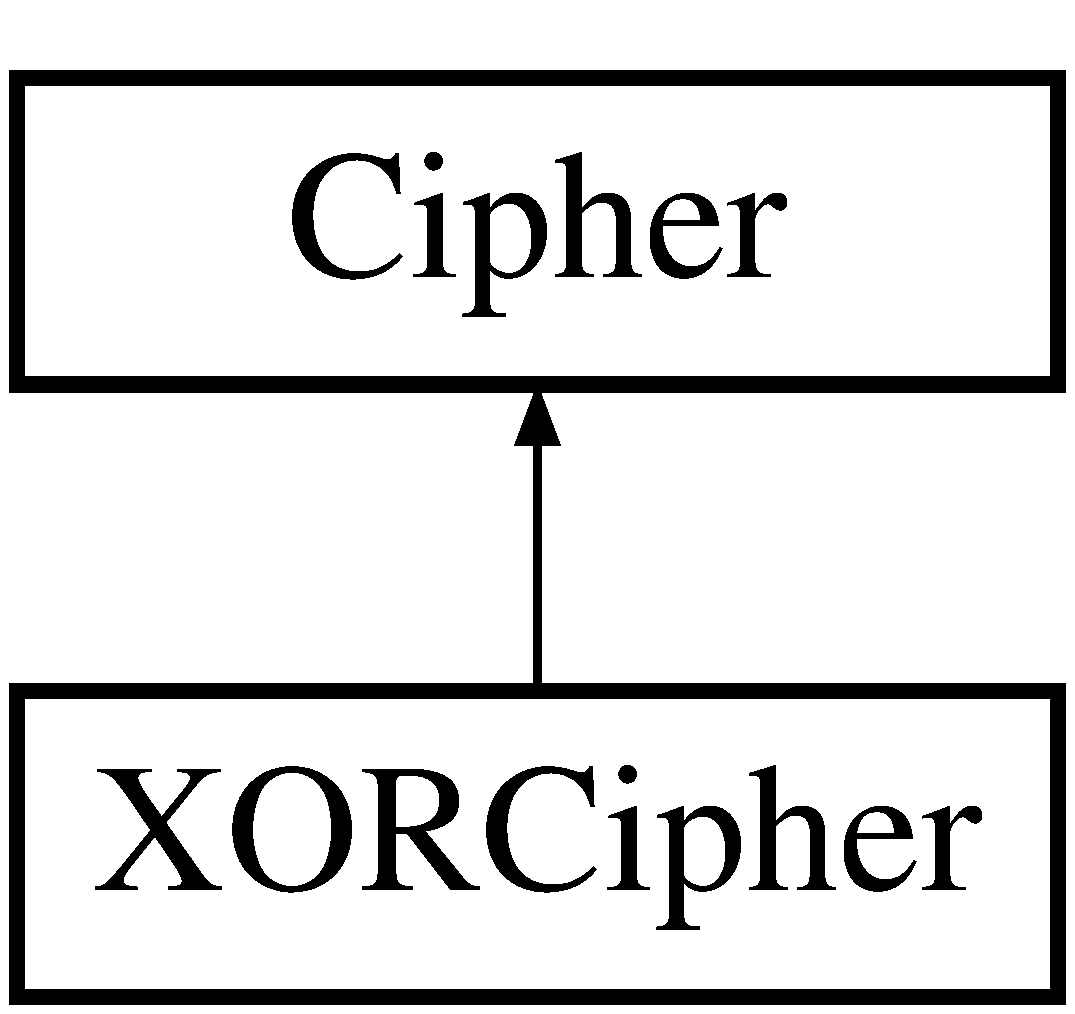
\includegraphics[height=2.000000cm]{class_x_o_r_cipher}
\end{center}
\end{figure}
\subsection*{Publikus tagfüggvények}
\begin{DoxyCompactItemize}
\item 
char $\ast$ \hyperlink{class_x_o_r_cipher_ac8ac09a4fcac428386935c31dea03768}{encrypt} (char $\ast$plain\+Text, char $\ast$cipher\+Key, int length)
\item 
char $\ast$ \hyperlink{class_x_o_r_cipher_ab3afeef39c53f0345163a6e46aac25b3}{decrypt} (char $\ast$cipher\+Text, char $\ast$cipher\+Key, int length)
\end{DoxyCompactItemize}


\subsection{Részletes leírás}
X\+OR titkos�t� oszt�ly. � v�gzi a X\+OR titkos�t�st �s visszafejt�st. 

\subsection{Tagfüggvények dokumentációja}
\mbox{\Hypertarget{class_x_o_r_cipher_ab3afeef39c53f0345163a6e46aac25b3}\label{class_x_o_r_cipher_ab3afeef39c53f0345163a6e46aac25b3}} 
\index{X\+O\+R\+Cipher@{X\+O\+R\+Cipher}!decrypt@{decrypt}}
\index{decrypt@{decrypt}!X\+O\+R\+Cipher@{X\+O\+R\+Cipher}}
\subsubsection{\texorpdfstring{decrypt()}{decrypt()}}
{\footnotesize\ttfamily char $\ast$ X\+O\+R\+Cipher\+::decrypt (\begin{DoxyParamCaption}\item[{char $\ast$}]{cipher\+Text,  }\item[{char $\ast$}]{cipher\+Key,  }\item[{int}]{length }\end{DoxyParamCaption})\hspace{0.3cm}{\ttfamily [virtual]}}

Az abstract oszt�ly virtu�lis visszafejt� met�dusa. A param�ter�l kapott �rt�ket a param�ter�l kapott titkos kulccsal visszafejti eredeti �llapot�ba.


\begin{DoxyParams}{Paraméterek}
{\em cipher\+Text} & A titkos�tott sz�veg \\
\hline
{\em cipher\+Key} & A titkos kulcs \\
\hline
{\em length} & A titkos�tott sz�veg hossza \\
\hline
\end{DoxyParams}
\begin{DoxyReturn}{Visszatérési érték}
A visszafejtett sz�veg 
\end{DoxyReturn}


Megvalósítja a következőket\+: \hyperlink{class_cipher_a39b1608e01f73f75ee248ef566aa44f9}{Cipher}.

\mbox{\Hypertarget{class_x_o_r_cipher_ac8ac09a4fcac428386935c31dea03768}\label{class_x_o_r_cipher_ac8ac09a4fcac428386935c31dea03768}} 
\index{X\+O\+R\+Cipher@{X\+O\+R\+Cipher}!encrypt@{encrypt}}
\index{encrypt@{encrypt}!X\+O\+R\+Cipher@{X\+O\+R\+Cipher}}
\subsubsection{\texorpdfstring{encrypt()}{encrypt()}}
{\footnotesize\ttfamily char $\ast$ X\+O\+R\+Cipher\+::encrypt (\begin{DoxyParamCaption}\item[{char $\ast$}]{plain\+Text,  }\item[{char $\ast$}]{cipher\+Key,  }\item[{int}]{length }\end{DoxyParamCaption})\hspace{0.3cm}{\ttfamily [virtual]}}

Az abstract oszt�ly virtu�lis titkos�t� met�dusa. A param�ter�l kapott �rt�ket a szint�n param�ter�l kapott titkos kulccsal titkos�tja.


\begin{DoxyParams}{Paraméterek}
{\em plain\+Text} & A titkos�tand� sz�veg \\
\hline
{\em cipher\+Key} & A titkos kulcs \\
\hline
{\em length} & A titkos�tand� sz�veg hossza \\
\hline
\end{DoxyParams}
\begin{DoxyReturn}{Visszatérési érték}
A titkos�tott sz�veg 
\end{DoxyReturn}


Megvalósítja a következőket\+: \hyperlink{class_cipher_a8a1970fdcb363529590299f14a6f2571}{Cipher}.



Ez a dokumentáció az osztályról a következő fájlok alapján készült\+:\begin{DoxyCompactItemize}
\item 
cipher.\+h\item 
cipher.\+cpp\end{DoxyCompactItemize}

%--- End generated contents ---

% Index
\backmatter
\newpage
\phantomsection
\clearemptydoublepage
\addcontentsline{toc}{chapter}{Tárgymutató}
\printindex

\end{document}
